\documentclass[final]{beamer} % beamer 3.10: do NOT use option hyperref={pdfpagelabels=false}!

%\documentclass[final,hyperref={pdfpagelabels=false}]{beamer} % beamer 3.07: get rid of beamer warnings

\mode<presentation>{\usetheme{dsmanchester}}

% Portrait, A0 poster. Set scale as desired, but 1.o3 gives easily readable text when printed.
\usepackage[orientation=landscape, size=a0, scale=1.2]{beamerposter}
\usepackage{booktabs}
\usepackage{caption}
\usepackage{subcaption}
\usepackage{adjustbox}
% Set height of page for use in arranging text boxes, after accounting for
% heading, footer etc. This is a bit of a hack, ideally latex should figure
% this out for itself!

\newcommand{\rpm}{\raisebox{.2ex}{$\scriptstyle\rpm$}}

\newlength{\columnheight}
\setlength{\columnheight}{841mm}
\setlength{\tabcolsep}{12pt}

                  
% Define the header information
\title{Unsupervised Task Discovery in Multi-Task Acoustic Modeling \\ \vspace{0.3em} Initial Findings}
\author{
  \textit{Josh Meyer}$^*$}
\institute{$*$ University of Arizona}


% Put any other packages or custom macros in here:



% Now start the actual poster
\begin{document}

% Header is automatically generated from the command defined in the theme
% file, the information above and the logos in the logo folder.


% Start of the body:
\begin{frame}
  \begin{columns}
    %% Leftmost column:
    \begin{column}{0.22\textwidth}
      % For some reason we need parbox to get it to arrange the boxes
      % with evenly spaced gaps
      \parbox[t][\columnheight]{.9\textwidth}{
        \begin{block}{Abstract}
          \begin{itshape}   % italic abstract
            \begin{itemize}
            \item Multi-Task Learning works (esp. in low-resource)
            \item However, tasks are hard to make
            \item Better to discover tasks automatically
            \item Experiment with k-means on MFCCs
            \item Initial results
            \end{itemize}
          \end{itshape}
        \end{block}

        \vspace{.5cm}

        \begin{figure}[!htbp]
          \centering
          \minipage{.66\textwidth}
          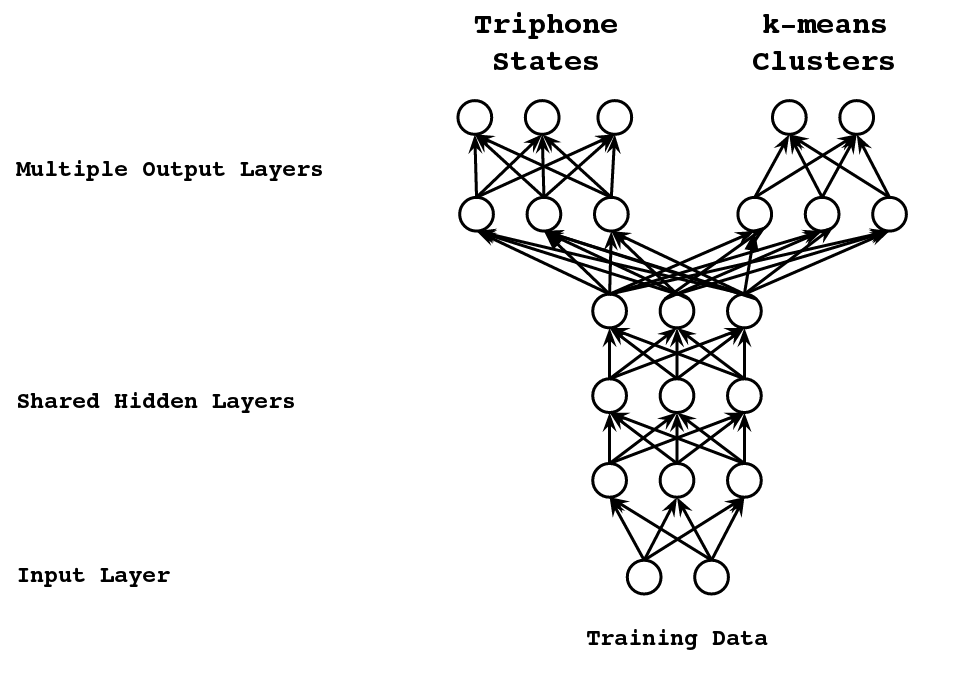
\includegraphics[width=\linewidth]{figs/heigold-2013-dnn-c.png}
          \caption{Multi-Task Learning Architecture}
          \label{fig:mtl-dnn}
          \endminipage\hfill
        \end{figure}
        
        \vspace{.5cm}

        \begin{block}{\boxnumber Background}
          \begin{itemize}
          \item Multi-Task Learning in Acoustic Modeling
            \begin{itemize}
            \item Multilingual
              \begin{itemize}
              \item new language == new task
              \end{itemize}
            \item Monolingual
              \begin{itemize}
              \item new linguistic encoding == new task
                \item Monophones vs. Triphones
              \end{itemize}
            \end{itemize}     
          \end{itemize}
        \end{block}
        \vspace{.5cm}

        \vspace{.5cm}

        \begin{figure}[!htbp]
          \centering
          \minipage{.8\textwidth}
          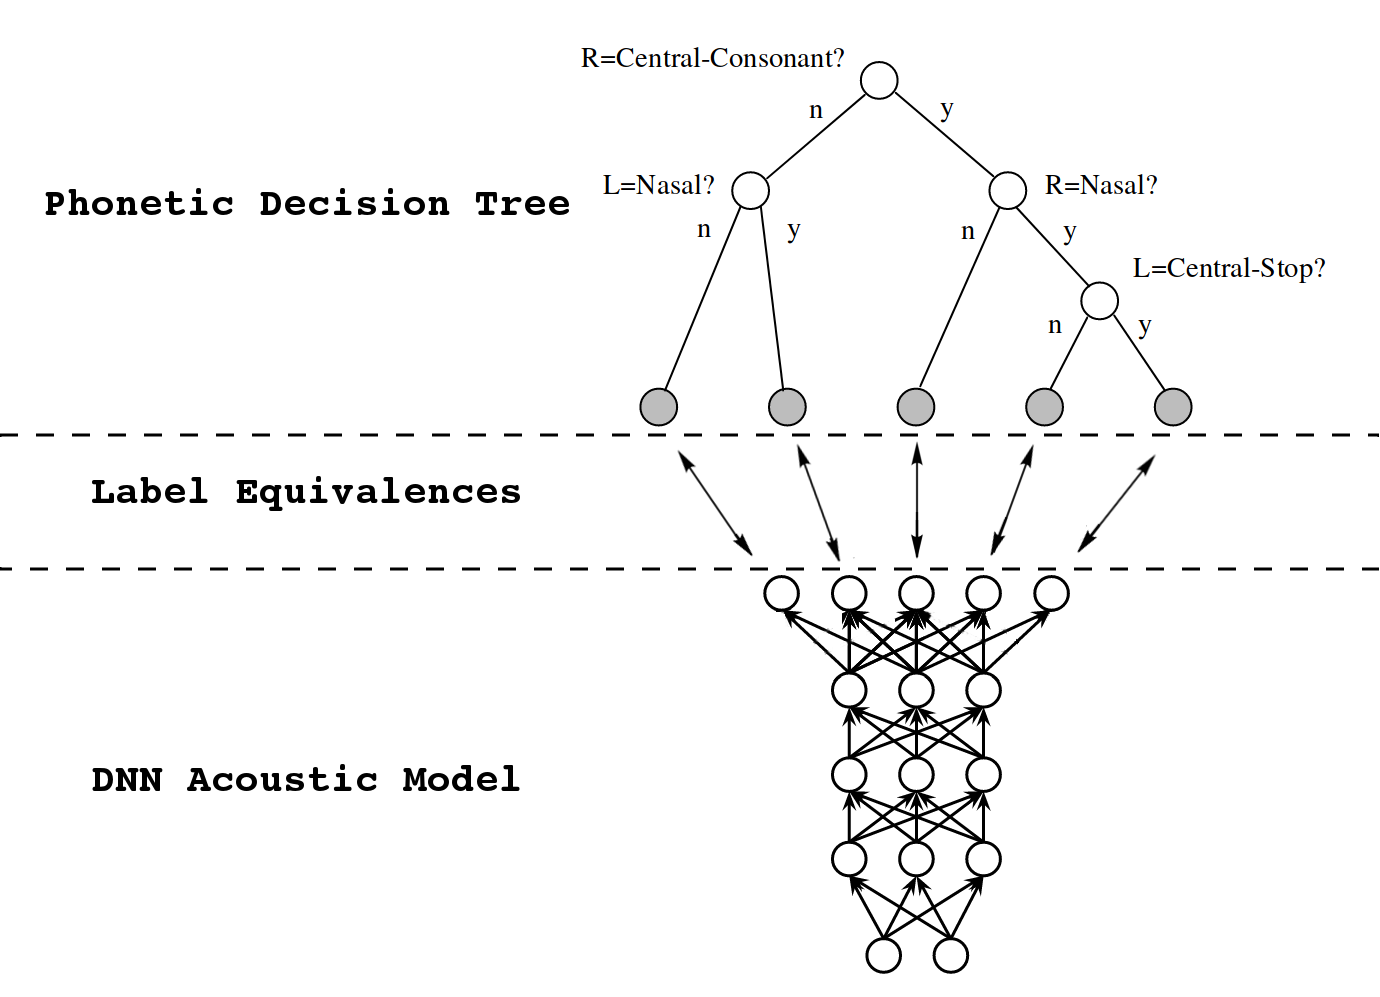
\includegraphics[width=\linewidth]{figs/tree-net.png}
          \caption{Label Correspondance of Decision Tree / DNN }
          \label{fig:mtl-dnn}
          \endminipage\hfill
        \end{figure}

        \vspace{.5cm}
      } % end of parbox
    \end{column}

    %% Next column:
    %% ============================================================
    \begin{column}{0.22\textwidth}
      \parbox[t][\columnheight]{.9\textwidth}{
        \vspace{.5cm}
        \begin{block}{\boxnumber Alignment}
          \begin{itemize}
          \item Feature Extraction
            \begin{itemize}
            \item 13 PLP features, 25ms Hamming windows, 10ms shift, 16 frame left-context \& 12 frame right-context, CMVN
            \end{itemize}
          \item GMM Alignment
            \begin{itemize}
            \item Monophones: 1,000 Gaussians, 25 iterations EM // Triphones: 2,000 leaves \& 5,000 Gaussians, 25 iterations EM
            \end{itemize}
          \end{itemize}
        \end{block}
  
        \vspace{.5cm}

        \begin{figure}[!htbp]
          \centering
          \minipage{.8\textwidth}
          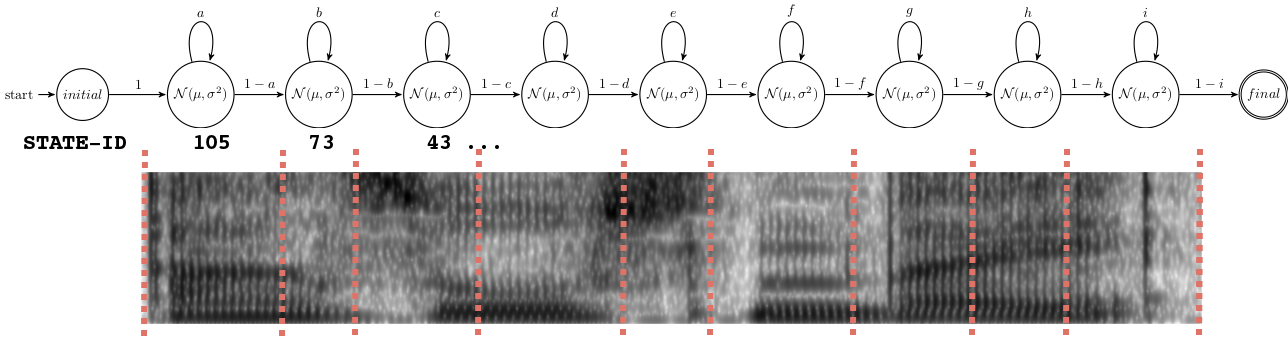
\includegraphics[width=\linewidth]{figs/aligned.png}
          \caption{GMM-aligned training examples}
          \endminipage\hfill
        \end{figure}
        
        \vspace{.5cm}
        
        \begin{block}{\boxnumber Clustering}
                    
          \begin{itemize}
          \item k-means Clustering
            \begin{itemize}
            \item A set number of clusters is discovered via TensorFlow's standard k-means clustering.
            \end{itemize}
          \end{itemize}
        \end{block}

        \vspace{.5cm}
        
        \begin{figure}[!htbp]
          \centering
          \minipage{.8\textwidth}
          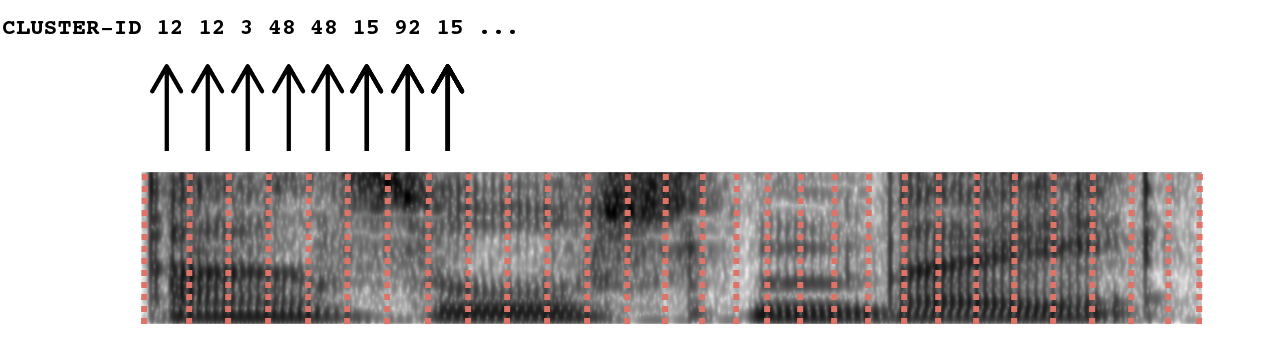
\includegraphics[width=\linewidth]{figs/clustered.png}
          \caption{k-means clustered training examples}
          \endminipage\hfill
        \end{figure}
        
        \vspace{.5cm}
        
        \begin{block}{\boxnumber Mapping Triphone States $\rightarrow$ Clusters}          
          \begin{itemize}
          \item Mapping triphone states $\rightarrow$ k-means clusters
            \begin{itemize}
            \item All training examples aligned to triphone state are mapped to most common k-means cluster.
            \end{itemize}
          \end{itemize}
        \end{block}

        \vspace{.5cm}
        
        \begin{figure}[!htbp]
          \centering
          \minipage{.8\textwidth}
          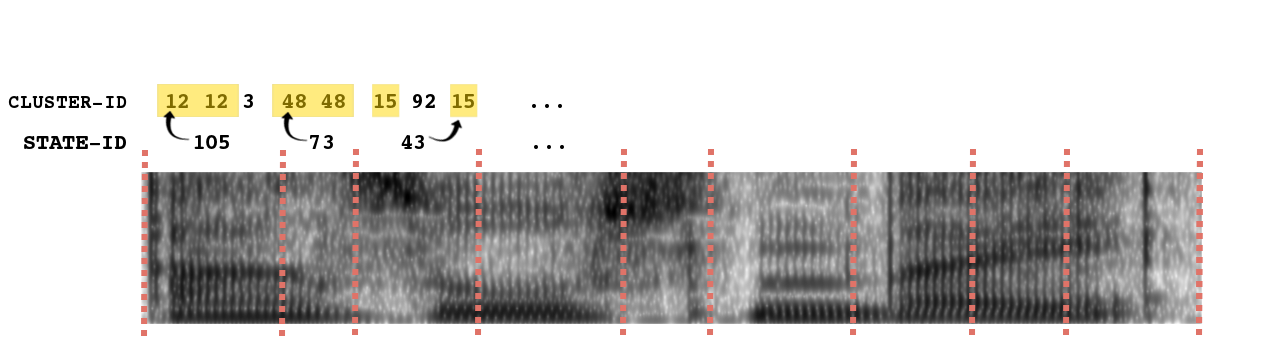
\includegraphics[width=\linewidth]{figs/mapped.png}
          \caption{GMM-aligned training examples}
          \endminipage\hfill
        \end{figure}
        
        \vspace{.5cm}  

        \begin{block}{\boxnumber DNN Training}          
          \begin{itemize}    
          \item DNN Acoustic model training
            \begin{itemize}
            \item 11 hidden layers, $ReLU$ activations
            \item 5-epochs
            \item $\alpha_{initial}=0.0015$ $\rightarrow$ $\alpha_{final}=0.00015$
            \item Each task has penultimate + ultimate output layer
            \end{itemize}
          \end{itemize}
        \end{block}
        \vspace{.5cm}
       
      } % end of parbox
    \end{column}
    
    %% Next column:
    %% ============================================================
    \begin{column}{0.22\textwidth}
      \parbox[t][\columnheight]{.9\textwidth}{

        \vspace{.5cm}               % automatically nicely spaced out.

        \begin{block}{\boxnumber Preliminary Results}
          \begin{table}[!htbp]
            \centering
            \caption{Word Error Rates (WER\%)}
            \label{tab:results}
            \begin{adjustbox}{width=.9\textwidth}
              \begin{tabular}{lccc}
                \toprule
                & \multicolumn{3}{c}{ \textit{Weighting Scheme ($(1-\alpha)*main + \alpha*aux$)}}\\
                & $\alpha = .9 $ & $\alpha = .8 $ & $\alpha = .7 $\\
                \midrule
                Single Task Baseline  &  \multicolumn{3}{c}{$57.10 $ \raisebox{.33\height}{\footnotesize{$\pm 3.25$}}}     \\
                \textbf{+ 256 k-means cluster targets}  &  $57.71 $ \raisebox{.33\height}{\footnotesize{$\pm 1.59$}}   &  $57.27 $ \raisebox{.33\height}{\footnotesize{$\pm 1.60$}}     & $57.89 $ \raisebox{.33\height}{\footnotesize{$\pm 1.29$}} \\
                \textbf{+ 1024 k-means cluster targets}   & $57.74 $ \raisebox{.33\height}{\footnotesize{$\pm 3.17$}}    & $57.08 $ \raisebox{.33\height}{\footnotesize{$ \pm 2.62$}}    & $57.77 $ \raisebox{.33\height}{\footnotesize{$\pm .79$}}  \\
                \textbf{+ 4096 k-means cluster targets}   &  $57.13 $ \raisebox{.33\height}{\footnotesize{$\pm 2.45$}}  & $57.76 $ \raisebox{.33\height}{\footnotesize{$\pm 1.61 $}}   &   $57.72 $ \raisebox{.33\height}{\footnotesize{$\pm .64$}}  \\
                \midrule
                \bottomrule
              \end{tabular}
            \end{adjustbox}
          \end{table}
        \end{block}

        
        \vspace{.5cm}


        \begin{figure}
          \centering
          \begin{subfigure}{.5\textwidth}
            \centering
            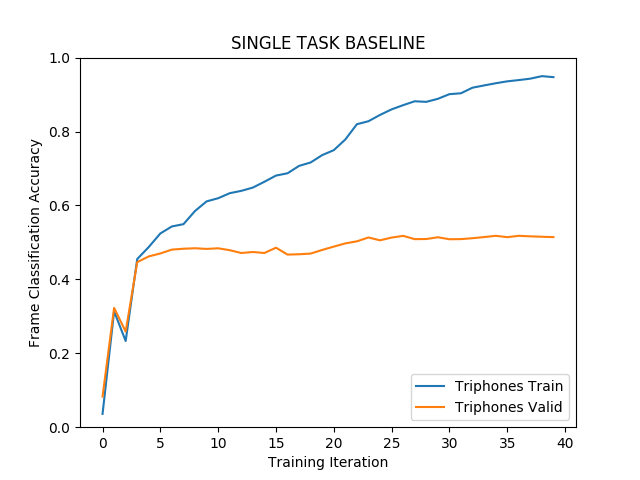
\includegraphics[width=.95\linewidth]{figs/baseline.png}
            \caption{Single Task Baseline}
            \label{fig:sub1}
          \end{subfigure}%
          \begin{subfigure}{.5\textwidth}
            \centering
            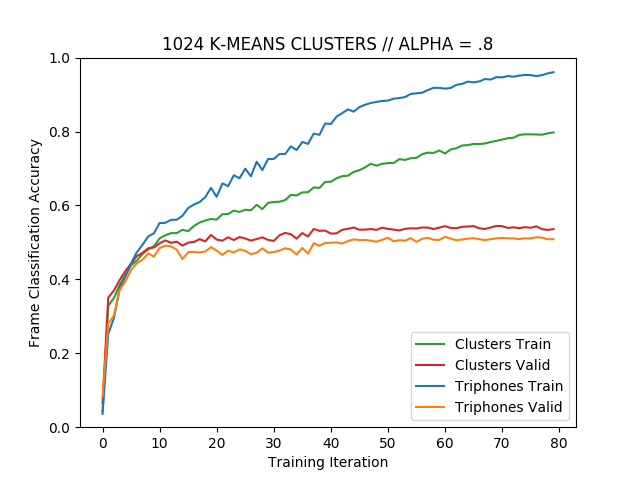
\includegraphics[width=.95\linewidth]{figs/1024-clusters.png}
            \caption{1024-clusters | Alpha == 0.8}
            \label{fig:sub2}
          \end{subfigure}
          \caption{Frame-level Accuracy | LOSS = (1-alpha)*MAIN + (alpha)*AUX }
          \label{fig:test}
        \end{figure}

        
        \vspace{.5cm}

                \begin{block}{\boxnumber Preliminary Results}
          \begin{table}[!htbp]
            \centering
            \caption{Word Error Rates (WER\%)}
            \label{tab:results}
            \begin{adjustbox}{width=.9\textwidth}
              \begin{tabular}{lccc}
                \toprule
                & \multicolumn{3}{c}{ \textit{Weighting Scheme ($1*main + \alpha*aux$)}}\\
                & $\alpha = .9 $ & $\alpha = .8 $ & $\alpha = .7 $\\
                \midrule
                Single Task Baseline  &  \multicolumn{3}{c}{$57.10 $ \raisebox{.33\height}{\footnotesize{$\pm 3.25$}}}     \\
                \textbf{+ 256 k-means cluster targets}  &  $ $ \raisebox{.33\height}{\footnotesize{$\pm $}}   &  $ $ \raisebox{.33\height}{\footnotesize{$\pm $}}     & $ $ \raisebox{.33\height}{\footnotesize{$\pm $}} \\
                \textbf{+ 1024 k-means cluster targets}   & $ 57.58$ \raisebox{.33\height}{\footnotesize{$\pm 2.68$}}    & $ 56.86$ \raisebox{.33\height}{\footnotesize{$\pm 1.11$}}    & $57.19  $ \raisebox{.33\height}{\footnotesize{$\pm 1.31$}}  \\
                \textbf{+ 4096 k-means cluster targets}   &  $57.78 $ \raisebox{.33\height}{\footnotesize{$\pm 2.36$}}  & $ 57.51$ \raisebox{.33\height}{\footnotesize{$\pm  2.65$}}   &   $ 57.03$ \raisebox{.33\height}{\footnotesize{$\pm 1.48$}}  \\
                \midrule
                \bottomrule
              \end{tabular}
            \end{adjustbox}
          \end{table}
        \end{block}        

        \vspace{.5cm}


        \begin{figure}
          \centering
          \begin{subfigure}{.5\textwidth}
            \centering
            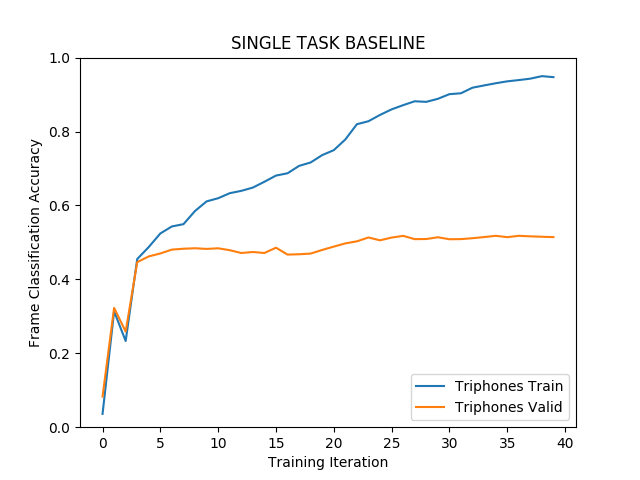
\includegraphics[width=.95\linewidth]{figs/baseline.png}
            \caption{A subfigure}
            \label{fig:sub1}
          \end{subfigure}%
          \begin{subfigure}{.5\textwidth}
            \centering
            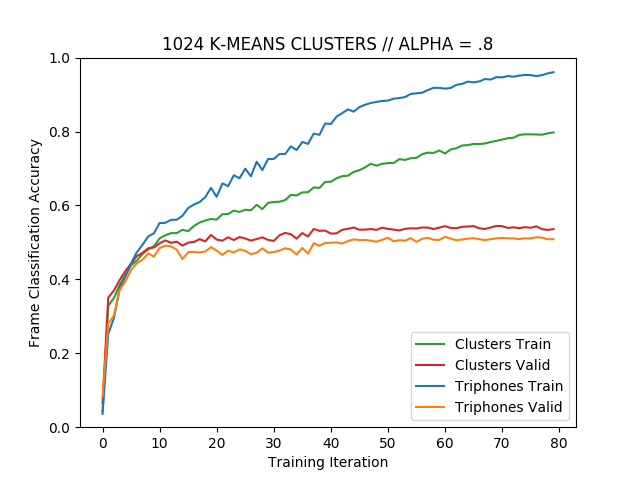
\includegraphics[width=.95\linewidth]{figs/1024-clusters.png}
            \caption{A subfigure}
            \label{fig:sub2}
          \end{subfigure}
          \caption{A figure with two subfigures}
          \label{fig:test}
        \end{figure}
        
      } % end of parbox
    \end{column}



    
    %% Next column:
    %% ============================================================
    \begin{column}{0.22\textwidth}
      \parbox[t][\columnheight]{.9\textwidth}{

        \vspace{.5cm}               % automatically nicely spaced out.
        
        \begin{block}{\boxnumber Cluster Contents: A Qualitative Discussion}
          
          \begin{itemize}
          \item 1024 clusters in TF
          \item 672 leaves in Kaldi
            
          \item 185 new labels after mapping
            \begin{itemize}
            \item 123 / 185 are interpretable
            \end{itemize}
          \item 101 of new labels contain mixed phonemes
            \begin{itemize}
            \item 39 / 101 contained either only vowels or only consonants
            \end{itemize}
          \item 84 of new labels contain one phoneme
            \begin{itemize}
            \item 9 / 84 contained more than one triphone of phoneme
            \end{itemize}
          \end{itemize}
          
          \begin{table}[!htbp]
            \centering
            \caption{Discovered intelligible Phoneme Clusters}
            \label{tab:results}
            \begin{adjustbox}{width=.5\textwidth}
              \begin{tabular}{llrr}
                \toprule
                \multicolumn{2}{c}{Vowels} &  \multicolumn{2}{c}{ Consonants} \\
                \midrule
                a  j & a  u  &   k  r &     g n m \\
                a  o & a  ih  &    k p  &    s sh ch\\
                e  j & e  ih & r ng & t k s p \\
                e  y &o  u & d ch & m ng\\
                u  ih  y   & u  ih & t k & t k h\\
                i  e  y &o  ih & d z&t k s \\
                a  e  oe  j ih & j ih & l z  & t ch d\\
                a  ih  o  u  y &  &  n p & t k zh b  \\
                &&& t g b s sh z zh \\
                \bottomrule
              \end{tabular}
            \end{adjustbox}
          \end{table}
          
        \end{block}
        \vspace{.5cm}
        
        
        \begin{block}{\boxnumber Acknowledgements}
          \footnotesize{This material is based upon work supported by the National Science Foundation Graduate Research Fellowship under Grant No. (DGE-1746060). Any opinion, findings, and conclusions or recommendations expressed in this material are those of the authors(s) and do not necessarily reflect the views of the National Science Foundation.}
        \end{block}
        \vspace{.5cm}
        
      } % end of parbox
    \end{column}


    
  \end{columns}
\end{frame}

\end{document}
